% !TEX spellcheck = uk_en
\documentclass[main.tex]{subfiles} 

\begin{document}

\section*{Undervisningsopplegget}
\label{sec:1}

Vi, lærerstudentene, observerte elevene fra 8. klasse i både naturfagtimer og matematikk timer. Elevenes faglig bakgrunn er varierende, 
klassen har en gjennomsninttelig fordeling av fagelig sterke og faglig svake elever. Før undervisningsopplegget ble utført observerte vi 
elevene gjennom flere timer, blant annet
i en naturfag time. I denne timen brukte elevene mikroskop for å studere diverse celleprøver, blant annet fra deres egen munn. Timen startet
med repitisjon av begreper om celler og mikroskop. Elevene ble fordelt i grupper på 3-4 stykker, og læreren gikk rundt og veiledet alle gruppene, 
deriblant hjalp læreren med å innstille mikroskopene til elevene slik at de endte opp med riktig fokus. Læreren gjennomgikk deretter 
felles med elevene med et mikroskop som var koblet til datamaskinen. Bildet fra mikroskopet ble projisjert på lystavlen i laboratoriet. 
Dette inspirerte oss til å bruke en tilsvarende opplegg til å strukturere vår egen undervisningstime(r), og faller under det John Dewey (1859 - 1952)
kaller utforskende arbeidsmåter, \citeA{rogs13}, \citeA[kap. 1]{knai11}.

Undervisningssekvesene vi har forberedt har til hensikt å utfylle følgende \textbf{kompetansemål i læreplanen}
\newline
\newline
\emph{Forskerspiren} :
\begin{itemize}
\vspace{-2mm}
\item formulere testbare hypoteser, planlegge og gjennomføre undersøkelser 
av dem og diskutere observasjoner og resultater i en rapport
\end{itemize}
\emph{Mangfold i naturen} :
\begin{itemize}
\vspace{-2mm}
\item beskrive oppbygningen av dyre- og planteceller og forklare hovedtrekkene i fotosyntese og celleånding
\vspace{-5mm}
\item gjøre rede for celledeling og for genetisk variasjon og arv
\end{itemize}
Undervisningseksvensene er fordelt over 3 skoletimer over 2 uker. Opplegget ble laget i henhold til forutsetningene til elevene og deres bakgrunn
basert på våre observasjoner og tilbakemeldinger fra veileder. Dette opplegget utførte jeg alene, med veileder og en medstudent som observatører. 
De bidro også i blant med å gi personlig/gruppe veiledning når elevene jobbet enten selvstendig eller sammen i grupper.

\subsection*{Microsoft OneNote}

OneNote er en dataprogram som lar brukere inntaste enten fra tastatur, eller kan brukes sammen med en smartboard
med en stylus til å føre håndskrevne notater. Bilder, tabeller og videor kan settes inn i notatene. Sidene i notatene blir
lagret automatisk og organisert i seksjoner i notatboken.

I undervisningen ble OneNote brukt til de første to timene. Isteden for tavleundervisning, ble OneNote brukt til å føre 
forelesningsnotater, og i et av sekvensene ble digitalerepresentasjoner brukt til å fremstille organsystemer 
(se figurene \ref{fig:notat1} - \ref{fig:notat2}). Disse notatene blir lagret på nettskyen, som elevene kan ha 
lesetilgang til fra sine private koblinger. Elevene har ikke tilgang til egne maskiner i timene (siden dette strider
mot skolens ordensregler om bruk av mobiler og andre verktøy i timen), med mindre en så-kalt laptoptralle blir hentet 
til klassen av underviseren. En slik tralle inneholder flere pcer som elevene låner midlertidig for å utføre skolearbeid. 
I våre timer valgte vi å ikke benytte laptoptrallen siden undervisningen ble ført på lystavlen og elevene ble isteden bedt 
om å ta skriftelige notater. Noe som viser seg er ikke normen, med mindre elevene blir eksplisitt bedt om å ta notater. 
Dette vil vi senere gå nærmere inn på når vi analyserer undervisningssekvensene.

\begin{figure}[h!]
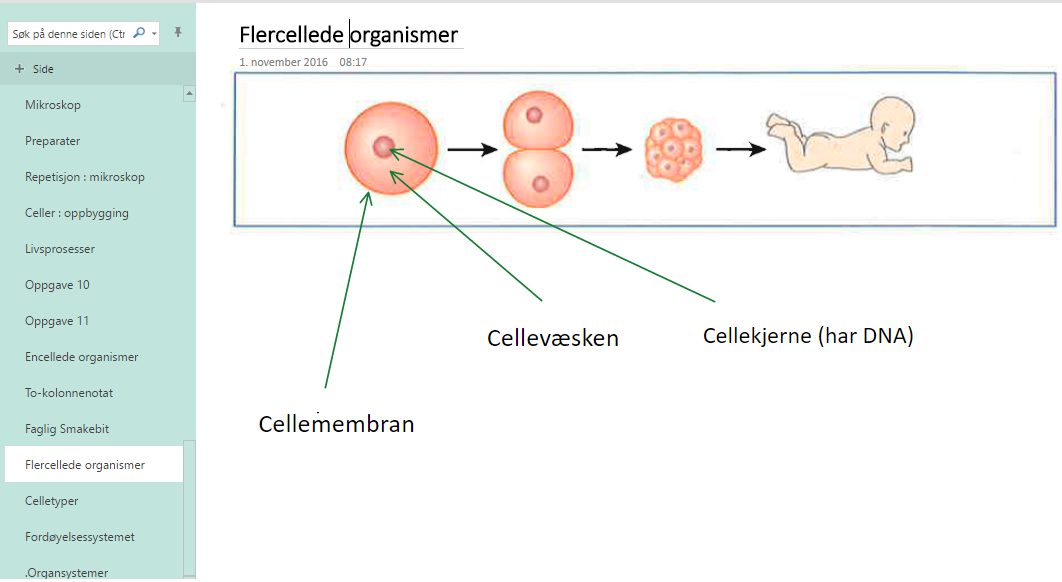
\includegraphics[scale = 0.6]{../figures/onenote_flercellet.png}
\caption{notat 1}
\label{fig:notat1}
\end{figure}

\begin{figure}[h!]
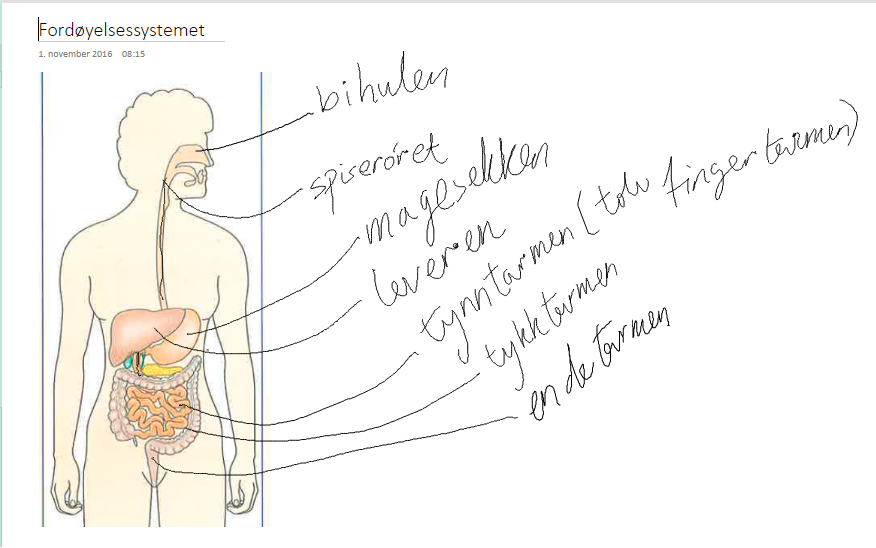
\includegraphics[scale = 0.6]{../figures/onenote_fordoyelse.png}
\caption{notat 2}
\label{fig:notat2}
\end{figure}

\subsection*{1.time}

Hensikten med denne timen var å oppsumere det elevene hadde lært hittil om celler og levendeorganismer, og
innføre nytt tema om encellede organismer. Timen startet med repetisjon av det elevene hadde lært fra sine
tidligere timer, deriblant om mikroskop og cellestruktur. 
I denne forbindelse ble tokolonnenotatet tatt i brukt (se vedlegg : \ref{sec:tokolonnenotat}). 

\subsection*{2.time}


\subsection*{3.time}

\end{document}